\chapter{Hiperboliczność}

\section{11.12.2024}{Przestrzenie hiperboliczne}

Na płaszczyźnie hiperbolicznej $\Hyp^2$ okrąg wpisany w trójkąt ma promień $r\leq\ln(1+\sqrt{2})$, które to ograniczenie nie zależy od długości boku trójkąta.

\begin{center}
  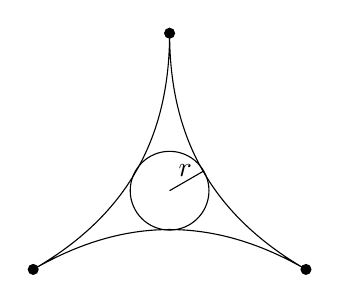
\begin{tikzpicture}
    \fill(90:2) circle (2pt);
    \fill(-30:2) circle (2pt);
    \fill(210:2) circle (2pt);

    \draw (90:2) to[out=-90, in=30] (210:2) to[out=30, in=150] (-30:2) to[out=150, in=-90] (90:2);
    \draw (0,0) circle (.5);
    \draw (0,0)--(30:.5);
    \node at (.2, .25) {$r$};
  \end{tikzpicture}
\end{center}

\begin{definition}{}{}
  Geodezyjna przestrzeń metryczna $(X, d)$ jest \buff{hiperboliczna} (w sensie Gromowa), gdy istnieje $\delta\geq 0$ taka, że każdy trójkąt geodezyjny w $X$ jest $\delta$-szczupły.
\end{definition}

Mówimy, że trójkąt jest $\delta$ szczupły, jeśli odległość dowolnego punktu z jednego boku do pozostałych krawędzi jest nie większa niż $\delta$. To znaczy, że krawędź zawiera się w sumie $\delta$-otoczeń pozostałych dwóch boków.
\begin{center}

  \tikzmath{\rad = .8;}
  \begin{tikzpicture}
    \filldraw[ultra thick, draw=blue, fill=blue!70, opacity=.6] ($(90:2)+(-\rad, 0)$) 
        to[out=-90, in=150] ($(-30:2)+({\rad*cos(-120)}, {\rad*sin(-120)})$)
        to[out=-30, in=-120] (-30:{2 + \rad})
        to[out=60, in=-30] ($(-30:2)+({\rad*cos(60)}, {\rad*sin(60)})$)
        to[out=150, in=-90] ($(90:2)+(\rad,0)$)
        to[out=90, in=0] (90:{2 + \rad})
        to[out=180, in=90] ($(90:2)+(-\rad,0)$);
    
    \begin{scope}[xscale=-1]
    \filldraw[ultra thick, draw=orange, fill=orange!70, opacity=.6] ($(90:2)+(-\rad, 0)$) 
        to[out=-90, in=150] ($(-30:2)+({\rad*cos(-120)}, {\rad*sin(-120)})$)
        to[out=-30, in=-120] (-30:{2 + \rad})
        to[out=60, in=-30] ($(-30:2)+({\rad*cos(60)}, {\rad*sin(60)})$)
        to[out=150, in=-90] ($(90:2)+(\rad,0)$)
        to[out=90, in=0] (90:{2 + \rad})
        to[out=180, in=90] ($(90:2)+(-\rad,0)$);
    \end{scope}

    \draw (90:2)--($(90:2)+(-\rad, 0)$);
    \node at ($(90:2)+({-.5*\rad}, 0)+(0, .3)$) {$\delta$};

    \fill(90:2) circle (2pt);
    \fill(-30:2) circle (2pt);
    \fill(210:2) circle (2pt);

    \draw (90:2) to[out=-90, in=30] (210:2) to[out=30, in=150] (-30:2) to[out=150, in=-90] (90:2);
  \end{tikzpicture}
\end{center}

Hiperboliczność w sensie Gromowa jest \buff{nizmiennikiem quasi-izometrii} geodezyjnych przestrzeni metrycznych.

\begin{definition}{}{}
  Skończenie generowalna grupa $G$ jest \buff{hiperboliczna}, gdy jej dowolny graf Cayleya $C(G,S)$ jest hiperboliczny.
\end{definition}

\begin{example}[m]
  \item $\Hyp^2$ i $\Hyp^n$ dla $n\geq 2$
  \item Drzewa (są $0$-hiperboliczne), a co za tym idzie grupy wolne i wirtualnie wolne. 
  \item Grupa podstawowa $\pi_1M$, gdzie $M$ jest zamkniętą przestrzenią o ujemnej krzywiźnie. Wtedy $\pi1_M\acts \widetilde{M}$ na nakryciu uniwersalnym w sposób geometryczny. Nakrycie to jest przestrzenią zupełną o krzywiźnie $-a^2<K<-b^2$.
  \item Grupy losowe, grupy małych skreśleń.
\end{example}

\begin{fact}{twierdzenie kombinacyjne}{}
  Grupy hiperboliczne są zamknięte na produkty wolne z amalgamacją względem
  \begin{itemize}
    \item podgrup skończonych
    \item podgrup maksymalnych cyklicznych
    \item podgrup quasi-izometrycznie włożonych i melnormalnych
  \end{itemize}
\end{fact}

Niehiperboliczne są grupy 
\begin{enumerate}
  \item zawierające $\Z^2$ jako podgrupę
  \item zawierające zdystorsowaną podgrupę cykliczną
\end{enumerate}

\begin{fact}{}{}
  Każda grupa hiperboliczna $G$ ma skończony wymiar asymptotyczny, $\asdim(G)<\infty$.
\end{fact}

\begin{proof}
  Niech $G$ będzie grupą $\delta$-hiperboliczną. Ustalmy $r>0$ i bez straty ogólności możemy założyć, że $r>\delta$. Będziemy konstruować jednostajnie ograniczone pokrycie $G$ o uniwersalnie (niezależnie od $r$) ograniczonej $r$-krotności.

  Ustalmy graf Cayleya $C(G,S)$ i weźmy dowolny punkt ze sfery $v\in S_{m\cdot 5r}(e)$ o środku w elemencie neutralnym $G$. Zdefiniujmy zbiór 
  $$U_v:=\{z\in G\;:\;(m+1)5r\leq d(e, z)\leq (m+2)5r,\;v\text{ leży na pewnej geodezyjnej od }z \text{ do }e\}$$
  Zbiór $U_v$ jest zacieniony na rysunku niżej, a fragmenty przykładowych geodezyjnych od punktów $U_v$ do $e$ przechodzących przez $v$ są narysowane na pomarańczowo.
  \begin{center}
    \begin{tikzpicture}
      % \fill[opacity=.3, orange] (60:3) to[out=55, in=170] (40:5.5) to[out=130, in=-10] (80:5.5) to [out=-20, in=65] (60:3);
      %
      % \draw[orange, very thick] (45:5.5) to[out=180, in=60] (0,0);
      % \draw[orange, very thick] (60:5) -- (0,0);
      % \draw[orange, very thick] (70: 5.2) to[out=-90, in=60] (0,0);
      \draw[orange, very thick] (70:5.2) to[out=-90, in=62] (60:2);
      \draw[orange, very thick] (60:5)--(60:2);
      \draw[orange, very thick] (50:4) to[out=190, in=58] (60:2);

      \draw[orange, very thick, dashed] (60:2)--(0,0);

      \fill[opacity=.3, orange] (70:3) to[out=-20, in=140] (50:3) to[out=50, in=170] (40:5.5) to[out=130, in=-10] (80:5.5) to[out=-50, in=70] (70:3);
        
      \draw (0,0) circle (2);
      \draw (0,0) circle (3);
      \draw (0,0) circle (5.5);
      \fill (0,0) circle (2pt);
      \node at (.1,.3) {$e$};

      \draw (0,0)--(150:2) node[midway, above, rotate=150, scale=-1] {$m\cdot 5r$};
      \draw (0,0)--(200:3) node[midway, above, rotate=200, scale=-1] {$(m+1)5r$};
      \draw (0,0)--(230:5.5) node[midway, above, rotate=230, scale=-1] {$(m+2)5r$};

      \fill (60:2) circle (2pt);
      \node at ($(60:2)+(-.1,.2)$) {$v$};
    \end{tikzpicture}
  \end{center}

  Średnica $\diam U_v\leq 20\cdot r$, bo $U_r\subseteq B_{10r}(v)$. Rodzina zbiorów
  $$\mathcal{U}:=\{B_{5r}(e)\}\cup \{U_v\;:\;v\in B_{5mr}(e),\;m\geq 1\}$$
  mają zbiory o średnicy $\leq 20r$ oraz pokrywa ona całą grupę $G$.

  % Będziemy teraz szukali niezależnego od $r$ ograniczenia na $r$-krotność.
  Jeśli $|m_1-m_2|\geq 2$, to istnieją $v_1\in B_{5m_1r}(e)$ oraz $v_2\in B_{5m_2r}(e)$ takie, że $d(U_{v_1}, U_{v_2})\geq 5r$. To oznacza, że nie istnieje kula $B_r(x)$ przecinająca oba zbiory $U_{v_1}$ i $U_{v_2}$. Jeśli jakaś kula $B_r(x)$ przecina $U_{v_1}$, $U_{v_2}$, to $d(U_{v_1}, U_{v_2})\leq 2r$, więc istnieją $z_1\in U_{v_1}$ oraz $z_2\in U_{v_2}$ takie, że $d(z_1,z_2)\leq 2r$. Rozważmy przypadek, gdy $v_1,v_2\in S_{5mr}(e)$. Wtedy 
  {\large\color{red}NIE CHCE MI SIE}
  % \begin{center}
  %   \begin{tikzpicture}
  %
  %   \end{tikzpicture}
  % \end{center}


\end{proof}

\subsection{Brzeg Gromova}

Przypomnijmy, że promienie geodezyjne w $X$ o początku w $x_0$ to były izometryczne odwzorowania $\rho:[0,\infty)\to X$ takie, że $\rho(0)=x_0$.

Na geodezyjnej przestrzeni hiperbolicznej $X$ dwa promienie geodezyjne o wspólnym początku
\begin{itemize}
  \item są $\delta$-blisko siebie
    \begin{center}
      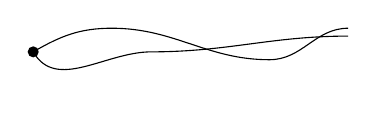
\begin{tikzpicture}
        \fill (0,0) circle (2pt);
        \draw (0,0) to[out=30, in=180] (1, .3) to[out=0, in=180] (3, -.1) to[out=0, in=180] (4, .3);
        \draw (0,0) to[out=-60, in=180] (1.5, 0) to[out=0, in=180] (4, .2);
      \end{tikzpicture}
    \end{center}
  \item albo od pewnego momentu uciekają od siebie do nieskończoności.
    \begin{center}
      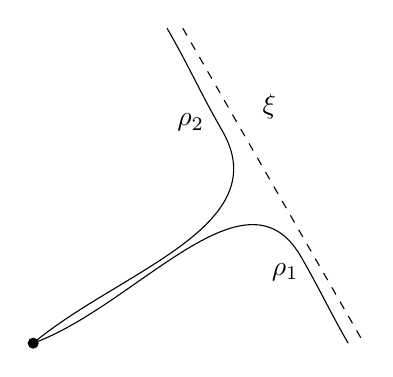
\begin{tikzpicture}
        \fill (-1,-1) circle (2pt);
        \draw (-1,-1) to[out=20, in=120] (2.4, 0.1) to[out=-60, in=120] (3, -1);
        \draw (-1,-1) to[out=40, in=-60] (1.4, 1.7) to[out=120, in=-60] (.7, 3);

        \draw[dashed] (.9, 3)--(3.2, -1);

        \node at (2.2, -.1) {$\rho_1$};
        \node at (1, 1.8) {$\rho_2$};
        \node at (2,2) {$\xi$};
      \end{tikzpicture}
    \end{center}
    $\xi$ na rysunku wyżej jest dwustronnie nieskończoną geodezyjną w $X$ taką, że $(\rho_1, \rho_2, \xi)$ jest $\delta$-szczupły. Wtedy \acc{produkt Gromova} jest w przybliżeniu $\langle \rho_1, \rho_2\rangle\approx d(x_0,\xi)$.
\end{itemize}

\begin{definition}{}{}
  Oznaczmy przez $\partial_\infty X$ zbiór promieni geodezyjnych o początku w punkcie $a$ wydzielony przez relację $\delta$-bliskości. Definiujemy na nim metrykę jako
  $$d_\infty([\rho_1], [\rho_2])\approx a^{-\langle \rho_1, \rho_2\rangle}$$
  dla odpowiedniego $a>1$.
\end{definition}

\begin{theorem}{}{}
  \begin{enumerate}
    \item $\partial_\infty X$ jako przestrzeń topologiczna nie zalęzy od wyboru $x_0$ oraz $a$
    \item Jeśli $f:X\to Y$ jest q.i. geodezyjnych przestrzeni metrycznych hiperbolicznych, to indukuje homeomorfizm $\widetilde{f}:\partial _\infty X\to \partial_\infty Y$
    \item Jeśli $f:X\to Y$ jest w.i. włożeniem, to indukuje $\widetilde{f}:\partial_\infty X\to \partial_\infty Y$ włożenie topologiczne.
  \end{enumerate}
\end{theorem}

\begin{example}[m]
  \item $\partial_\infty \Hh^2=S^1$, a także $\partial_\infty \Hh^n\cong S^{n-1}$
  \item Jeśli $M$ jest $n$-wymiarową rozmaitością o ujemnej krzywiźnie, to $\partial_\infty(\widetilde{M})=\partial_\infty\pi_1M\cong S^{n-1}$
\end{example}




